% 04-experiments.tex — truth: 本文件（2026-09-10 交割：R22 后全部正文修订直改 tex，原装配源 md 已冻结为历史设计稿，见其头部治理注记）
% 纪律: 4.1 数据集与三层口径协议(20/24 有效监督口径随行) / 4.2 实现细节+统计协议 / 4.3 主实验 E1-E6(每实验先声明 claim 句) /
% 4.4 对比研究(NTU 等价性段=成文块装配); tab2 真实 K9 列空缺如实标注; 内部路径/文件名禁入正文(ROUND2 发现#7)。
% 2026-11-16 回修（审查#3/#4/#11/#12）: 归因对照补 episode/budget 口径披露（60→10 界 vs 60→49 复制; 50/class 三臂 vs E6 n=30/100）;
%   E6 正文标注 n=3; tab:main caption 注明合成层全预算参照为单 run。逐 seed 配对比值入 supplementary (app:e6seeds)。
% 2026-11-16 P1 收官补位（写手·补充细节）: E1 同 episode（60→49）零重训界结果位预留（ssec:boundary 界段改为已注册待测
%   + tab:attribution-controls 增 60→49 界两行, \TODO 待回填）; E2/E3 协议与数字位、CIL 定位段入 supplementary
%   （app:mergebound49 / app:rebuildbudget / app:synthmigration / app:cil）。数字位禁编造, 由回填写手按实验产物回填。
% 2026-11-16 P1 回填（回填写手）: E1/E2/E3 出数, 数字源 runs/p1_sprint/{zerobound_6049,semantic_rebuild_1100,
%   split_addition_episode}/summary.json（reports/p1_sprint_evidence/ 有逐字节一致副本）——
%   tab:attribution-controls 60→49 界两行（68.04/67.97）与 E2 等预算三臂行（D′ 60.2% vs C′ 44.9%, 26.5×）已回填;
%   ssec:boundary/E6/E6-real-2 同步改"已测"; 60→10 与 60→49 两个 episode 不可互换的口径说明已强化。
% 2026-11-16 统稿: 新增 Reinforcement E3（split/addition 残余价值探测）与 E3b（k∈{10,25,50,100} 标注预算阶梯）
%   正文段 + tab:kladder——摘要/贡献1/结论所引 k 阶梯实验的正文载体; 协议全文在 supplementary app:synthmigration/app:kladder。
%   数字源 runs/p1_sprint/{split_addition_episode,k_ladder}/summary.json（reports/p1_sprint_evidence/ 有镜像）, 禁编造。
% 2026-11-16 P1 真实 tier 冻结编码器对照（统稿）: ssec:boundary 冻结对照 bullet 由"未运行/不赋值"改为已执行结果
%   （NTU120/UCF101/PanAf500 三臂 C/A/B；NTU60 未重跑, 沿用已报告 E9 参照 67.53±0.24）, tab:attribution-controls
%   增真实 tier 十行块, caption 同步; 协议全文在 supplementary app:frozenreal。数字源 runs/p1_sprint/{ntu120,ucf101,
%   panaf500}/summary.json, 与 reports/p5b-ntu120|p5b-ucf101|p23-panaf-retention-2026-09-07.json 逐位一致, 禁编造。
% 2026-11-16 终审回修（回修写手）: E9b/E9c 段补基准口径披露（NTU120=12,000-clip/60 类子集、UCF101=10,000-clip 子集,
%   各臂同口径; UCF101 官方 split1 val 仅 463 clips 一并注明）; tab:attribution-controls 表注同步 subset calibers
%   + 真实 tier 块无端到端微调臂的限定（frozen-vs-full-FT 对照仅合成层证据）; E3 decoupled 均值 45.8%→45.7%（三种子
%   0.4448/0.4345/0.4931 均值 0.45747 直接舍入, 消除两级舍入）。
% 2026-11-16 P1 头对头回填（写手·结果回填）: sec:comparison 新增 published-method 基线段 + tab:h2h——
%   AimCLR 线性评测（joint stream, 官方 LE recipe, in-house pretext 权重）10%/full = 66.71/74.30%,
%   监督 ST-GCN（端到端, 16 hidden channels, 0.84M 参数）10%/full = 66.52/83.46%, 与 E9 的 PSD 臂
%   （linear head 66.05 / semantic 67.53±0.24 / full 参照 74.45）同 10% 分层子集（seed 42, 4,009 clips）、
%   同 40,091 全量、同 16,487 验证集并排; 基线臂为单 run, 10% 差距仅作描述不下显著性结论。
%   数字源 runs/p1_sprint/{published_baseline_ntu60,supervised_stgcn_ntu60}/summary.json, 禁编造。
% 2026-11-16 P1 k 阶梯多种子回填: k=10/25/50 档补 seeds 43/44（同日补测, 初测单种子 readout 与合并三种子 summary 均存档）,
%   decoupled 45.29±0.16 / 59.08±2.52 / 65.06±1.33 / 72.41±0.00%（k=10/25/50/100, std ddof=0）,
%   边际 50.57/36.78/30.80/23.45pp; 数字源 runs/p1_sprint/k_ladder/summary.json（canonical 合并版）, 禁编造。
\section{Experiments}\label{sec:experiments}

\subsection{Datasets and the three-tier protocol}\label{sec:datasets}

Because no available dataset spans the scenarios our claims require (Section~\ref{ssec:rw-animal}), we evaluate under a three-tier protocol; numbers are never mixed within a comparison. The \emph{synthetic} tier serves pipeline shake-down and controlled ablations; the \emph{public-real} tier provides label-free and low-resource evaluation on real animal skeletons; the \emph{real-K9} tier (working-dog training footage) is reserved for the target domain and is not exercised in this study. Two further contexts are exercised under the same reporting rules and never pooled with the tiers: a \emph{synthetic-offset} variant of the synthetic tier (the same generator with Gaussian joint-coordinate noise, $\sigma{=}0.10$; its distribution fixed by a pre-registered diagnostic before any offset experiment ran) for the distribution-shift and warm-start studies, and public \emph{benchmarks} (NTU60/NTU120/UCF101 for human actions and PanAf500 for great apes) for the pre-registered E9-series cross-domain retention studies, each reported against its own full-budget reference. The working-dog pilot is nonetheless pre-registered before any data collection (protocol PSD-K9-PREREG-001, committed to the public review repository): a double-annotation agreement gate (Cohen's $\kappa\geq 0.60$), session-level splits, a single primary endpoint with a paired decision rule, and a no-redistribution clause for raw footage and derived skeletons.

The public-real tier draws on three sources. InterPet4D~\citep{peng2026interpet4d} provides 226 SMAL-fitted skeleton sequences of human--pet interactions (225 used; one all-NaN sequence excluded and listed) as the unlabeled stream for self-supervised pretraining and segmentation evaluation. From the official Animal Kingdom action-recognition lists~\citep{ng2022animalkingdom} we aggregate the canine-species subset: 329 videos (231 train / 98 test) with 34{,}772 frame-level annotation rows, for weak-supervision and behavior-classification evaluation. APTv2~\citep{yang2023aptv2} supplies a large pose pool (official: 2{,}749 clips, 41{,}235 frames; local inventory 41{,}179 images; consumed unlabeled) for expansion experiments. Skeletons are world-coordinate keypoint sequences of shape $T{\times}24{\times}3$ with a per-joint confidence channel. One structural caveat applies to every real-domain skeleton product: the dog-pose annotations never label four of the 24 graph slots (both eyes, withers, throat), so real-domain keypoints are topology-isomorphic with 20/24 effective supervision channels; the four dead channels are hard-masked at assembly and NaN-guarded downstream. A pre-registered expansion tier (v2; PSD-AKV2-PREREG-001, frozen before the build) re-extracts the same canine videos as multiple contiguous segments under a per-frame label-consistency gate, yielding 352 clips in an eight-class space; it serves as a parallel replication layer and never replaces v1 numbers (E7b).

\subsection{Implementation details}\label{sec:implementation}

All experiments run on a single consumer GPU (RTX 5060 Laptop, 8\,GB); self-supervised pretraining takes about 13 minutes for 120 epochs on InterPet4D, so the physics layer is reproducible without data-center resources. Pretraining uses a learning rate of 0.05, a queue of 1{,}024, and window length $T{=}64$; this is the first working setting, not the outcome of a systematic search. $k$-NN probes report 5-fold mean$\pm$std; end-to-end arms report seed-level dispersion (sample std, ddof~1), not confidence intervals; per-experiment seed choices are listed in the released experiment ledger and protocol files. Aggregate comparisons carry paired seed-level tests with Holm--Bonferroni correction within each experiment family (corrected values printed alongside), effect sizes with a random-baseline reference, and outliers explained rather than removed. The E9-series correction family (Section~\ref{sec:comparison}) consolidates eight paired tests: the pipeline-versus-linear gap tests on three tiers (NTU60, NTU120, UCF101; one-sample $t$ and Wilcoxon signed-rank each) plus the two external-SSL Wilcoxon tests. Each member's decision rule was fixed by its own pre-registered protocol before its run; the consolidated family was fixed before corrected inference entered this manuscript (dated 2026-09-07 in the repository). The PanAf500 gap is reported directionally and is not a family member (its arm distribution ties with the linear arm; raw $p=0.75$); adding it as a ninth member changes no corrected verdict, and under the narrower six-test gap-only sub-family every qualitative conclusion is unchanged. The head-to-head significance tests against the two published-method baselines (Table~\ref{tab:h2h}) are a separate post-hoc two-test family added in this revision (dated 2026-11-16/17 in the repository; per comparison, Welch is the primary test and Mann--Whitney the distribution-free sensitivity analysis, both Holm-corrected within the two-test family: the AimCLR gap reads raw $p{=}1.1\times10^{-6}$ Welch / $6.7\times10^{-4}$ Mann--Whitney, corrected $p{=}2.3\times10^{-6}$ / $1.3\times10^{-3}$); they are not members of the pre-registered E9-series family, and either family choice leaves the reported conclusions unchanged. Registration fixes decision rules before outcomes exist and prevents selective reporting; it did not catch the protocol-implementation errors we corrected (the oracle-label leakage of the initial end-to-end runs, Section~\ref{ssec:proto}), which came from internal adversarial review. Protocol freeze is evidenced by the dated commit history of the public review repository (tag \texttt{review-snapshot}); one protocol (the v2 expansion) and its results landed in the same repository batch, so its freeze is bookkeeping-grade evidence rather than third-party timestamping.

\subsection{Main results}\label{sec:main-results}

Table~\ref{tab:main} consolidates the main results across the three tiers plus the public human-domain benchmark used for implementation-equivalence verification; each numbered experiment below opens by stating the claim it tests; experiment labels follow the released experiment ledger (E5, the active-learning study, is reported as an exploratory finding in Section~\ref{sec:ablation}; E8, the budget curve, is folded into the E7 discussion). Claim tags: \textbf{C1} decoupled transition cost, \textbf{C3} pretraining value, \textbf{C4} unsupervised segmentation, \textbf{C5} anchor-guided semantic expansion, \textbf{C6} low-budget self-training behavior, \textbf{C7} active learning (exploratory negative); \textbf{C2} is the novelty claim, tested by the survey (supplementary material, Novelty survey matrix) rather than by an experiment.

\paragraph{E1: representation quality of the physics layer (C3).}
This experiment tests whether self-supervised pretraining on unlabeled quadruped skeletons yields discriminative dynamics representations. Using subject identity as a $k$-NN probe on InterPet4D (a proxy task that measures representation discriminability, not behavior accuracy), pretraining reaches \textbf{20.89\% $\pm$ 4.04\%} top-1 (sample std over the five folds) against an 8.33\% random baseline ($2.51\times$). The fold-level range is wide (15.56--26.67\%), attributed to the small number of sequences and subject diversity; a projection-head feature caliber yields 12.89\% ($1.55\times$), recorded in the released run report, and both calibers are valid views of the same encoder.

\paragraph{E2: unsupervised segmentation quality (C4).}
This experiment tests whether motion-word quantization cuts continuous streams into behavior-aligned proposals. Under a seeds pseudo-ground-truth protocol, boundary IoU against held-out annotations is \textbf{0.458 $\pm$ 0.049}, versus an equal-segment-count random-cut null of 0.323 $\pm$ 0.022 (Monte-Carlo expectation over 200 random cuts); boundary F1 is reported alongside (0.343 vs.\ the uniform-window 0.396), and the fixed-grid probe that is statistically on par with SMQ ($0.453 \pm 0.027$) is reported in Section~\ref{sec:ablation}.

Figure~1 of the supplementary material visualizes the resulting boundaries against the seed pseudo-ground-truth on the lowest- and highest-IoU episodes.

\paragraph{E3: anchor-guided label expansion (C5).}
This experiment tests whether a small rule-engine seed set expands toward taxonomy coverage via iterated pseudo-labeling. Anchor-guided prototype clustering reaches purity \textbf{0.5339} against a 0.3306 random-assignment baseline ($1.61\times$) and a 0.4858 all-majority baseline ($+4.8$\,pp; the binding comparison). Injecting 30\% label noise into the seeds degrades purity by only 3.1\,pp (0.5025$\pm$ 0.0063, still $1.52\times$ baseline), and enlarging the seed ratio from 25\% to 100\% changes purity by less than 1\,pp at $K\in\{5,10\}$ but costs 2.4\,pp at $K{=}14$, the best cell of the $k$-means sensitivity sweep (the main run is the deterministic class-mean configuration; full sweep in the released evidence archive). Prototype quality saturates early in seed ratio at small $K$, which is what makes a small seed budget practical.

\paragraph{E4: semi-supervised self-training on the public-real tier (C6).}
This experiment tests whether self-training converts pseudo-labeled coverage into usable classification under scarce labels. Iterating from round~0 to round~1 raises pseudo-label pool precision from 0.5125 to \textbf{0.691 $\pm$ 0.013} (a $+17.9$\,pp endpoint gain; the paired first-to-last statistic over all iterated rounds is $\Delta$ $+10.69\pm3.28$\,pp; the two numbers measure different spans and are both released); the precision-drop stopping rule fired after two consecutive degraded rounds, so round~1 is the reported operating point (Holm-corrected $p=0.090$ over the three-test family: the calibrated main first-to-last test, its no-consensus ablation, and the $\alpha{=}0$ control; released artifact \texttt{r16-holm-p04}; raw $p=0.030$, direction-consistent but not significant after family correction). Under the pre-registered partial-class protocol on the Animal Kingdom canine subset (4 of 12 classes pass the sample-size gate), a frozen-backbone classifier with a re-trained head reaches 41.5\% $\pm$ 5.9\,pp overall across three seeds (best seed 44.90\%), $1.66\times$ the 25\% uniform-random baseline ($1.80\times$ at the best seed). The per-class breakdown (watch 100\% / track 23.5\% / jump 0\% / stay 0\%) accompanies this number: the aggregate is dominated by class imbalance and interprets only in the four-class partial caliber (other public-real results carry their own class-space labels).

\paragraph{E7: end-to-end pipeline at small budget (C6; negative boundary).}
This experiment tests whether the complete pipeline, run end-to-end from a small annotation budget, approaches full supervision; it is the paper's principal negative boundary: on the only truly animal target domain exercised end-to-end (canine), the pipeline does not beat chance or a generic-SSL control (mechanism analysis in Section~\ref{ssec:boundary}). The arms follow a corrected protocol (revision R16 of the repository's experiment ledger): the final classifier is trained on seed ground-truth labels plus pseudo-labels for the confidence-filtered pool clips (never on pool ground truth), and iteration stops on convergence or the iteration budget (the precision-drop rule monitors pool precision against a rule-derived consensus reference, which this tier's label space does not provide; consuming true labels there would be oracle leakage; Section~\ref{ssec:proto}). On the 12-class-protocol public-real tier (9 classes with samples; 197 self-extracted clips; anchors and pool restricted to the training split, validation isolated), at 2 clips per class (18 of 141 training clips, $\approx$13\%; ten seeds) the pipeline reaches \textbf{9.8\% $\pm$ 7.5} top-1, at the tier's 11.1\% chance level, against 33.93\% under full supervision; the generic-SSL control reaches 15.2\% $\pm$ 5.1 and the scratch control 8.4\% $\pm$ 10.7; after per-tier Holm correction the only significant same-seed effects are on macro-F1, both favoring the generic-SSL arm ($5.1$\,pp at 2 clips/class, corrected $p=0.023$; $6.6$\,pp at 4, corrected $p=0.049$); warm-versus-scratch differences are not significant. The prototype-path consensus gate is inert on this taxonomy (no standing class; Section~\ref{ssec:proto}), so pool filtering reduces to the confidence margin alone. The iterated pseudo-labeling is the point of failure: pool pseudo-label precision, measured post hoc against training-split labels as a released diagnostic only, averages 0.11 across seeds, and a ground-truth-free per-round recalibration of the gate does not rescue it ($8.9$--$12.5\%$, three seeds). The negative boundary\footnote{An earlier internal protocol variant trained the final head on the pool clips' ground-truth labels and consumed oracle precision for stopping; its higher low-budget numbers were never published and are withdrawn. The correction, re-run evidence, and errata are documented in the released repository.}: on the canine tier, confidence-filtered pseudo-labels at a 13\% budget do not yield usable supervision, consistent with the label-alignment diagnosis of Section~\ref{sec:conclusion} (L9) and the saturated-scorer mechanism of E5 (Section~\ref{sec:ablation}). The supervised references and comparisons on this tier (E4, the five-arm study in Section~\ref{sec:comparison}) are unaffected, and the cross-domain retention evidence (E9) holds under the same protocol; Figure~\ref{fig:budget} collects the retention points across all exercised tiers. Section~\ref{ssec:boundary} consolidates this boundary with the E7b/E7c evidence.

\paragraph{E7b: pre-registered replication on the expanded v2 tier.}
To test the data-bottleneck attribution instead of asserting it, we pre-registered a multi-segment expansion of the public-real tier (PSD-AKV2-PREREG-001, frozen before the build): the same 329 canine videos re-extracted as up to four contiguous segments each under a per-frame label-consistency gate ($\geq$0.80), yielding 352 clips (256 train / 96 val) in an eight-class space (bark segments fail the gate). All low-budget arms rerun under the corrected pseudo-label protocol of E7 at ten seeds. Leakage boundary: the warm-start backbone was supervised on v1 training-split videos, and v2 adds new segments of the same videos to its training pool; validation videos remain disjoint, but any warm-arm advantage partly co-occurs with source-video exposure and is not fully attributable to the method alone. The frozen decision rule fires on raw top-1 ($+3.57$\,pp), but that gap is confounded by the class-space change (nominal chance rises from the 12-class $8.33\%$ to the 8-class $12.5\%$); we therefore add a same-space control (post-hoc): reweighting the v1 full-supervision arm's per-class accuracies over the eight classes v2 retains, on v1's validation clips, yields 25.96\% (released artifact \texttt{r12-holm-eightclass}; errata for its remaining blocks are documented in the released repository). This removes the chance-rate confound but not the clip-set difference, so the same-space rise is $+11.54$\,pp (above-chance margin $13.5\to25.0$\,pp; above-majority $-4.8\to+3.1$\,pp). Under this control the top-1 data are consistent with the data-bottleneck attribution, and macro-F1 moves the same way ($16.5\%$ to $19.3\%$). The raw endpoint is numerically sensitive: re-running the identical supervised reference with a different label encoding shifts it by 2.1\,pp ($37.50\to35.42$; two validation clips), so the raw margin above the $+3.0$\,pp line is within solver-path noise and the attribution rests on the same-space control, whose margin is an order of magnitude larger.

The corrected low-budget arms do not replicate the earlier end-to-end reading: at 2 clips/class where a class has training clips (14 of 256, $\approx$5.5\%; the sit class has none), the warm-start arm reaches 13.1\% $\pm$ 5.3, the generic-SSL arm 17.6\% $\pm$ 4.3, and the scratch arm 13.8\% $\pm$ 5.6, against a 12.5\% chance rate, near chance as on v1; at 4 clips/class (10.9\%, 28 of 256; plotted in Figure~\ref{fig:budget}) the warm arm reads 16.6\% $\pm$ 6.8, i.e.\ 44.2\% retention of the archived 37.50\% v2 full-budget reference, with generic-SSL at 14.6\%, ordered as at spc2; the only significant same-seed effect in this family is macro-F1, where the warm arm beats scratch ($+4.6$\,pp, all ten pairs, per-tier Holm-corrected $p=0.012$). v1 remains the primary tier; v2 is reported alongside, never merged. As a diagnostic control, we also end-to-end fine-tune the backbone on v2: full-budget fine-tuning reaches 32.99\% $\pm$ 3.94 top-1 (three seeds), \emph{below} the frozen-head reference on both metrics (top-1 37.50\% archived, 35.42\% under the re-encoding above; macro-F1 19.33 vs.\ 16.73); at 2 clips/class fine-tuning reaches 9.72\% $\pm$ 1.59, comparable to the near-chance pseudo-label arms. Both metrics agree that unfreezing does not help at this data scale: this is the full-budget frozen-versus-tuned comparison that the decoupled design prescribes.

\paragraph{E7c: skeleton-quality attribution (pre-registered).}
The negative boundary above leaves one attribution open: is the ceiling set by skeleton quality or by label alignment? We pre-registered the test (PSD-SA-PREREG-001, frozen before the run): re-extract all 197 public-real videos with a substantially stronger estimator, YOLO11x-pose~\citep{jocher2024yolo11} fine-tuned on the dog-pose benchmark (up to 100 epochs, early-stopped at 89; pose mAP50 0.834 versus the production extractor's smaller model; extractor-training logs released with the K9 training repository), and re-evaluate the full-supervision reference on identical clips, splits, and labels. The stronger skeletons do \emph{not} raise the ceiling: 30.36\% versus 33.93\% ($-3.57$\,pp, below the pre-registered $+3$\,pp line; verdict \textbf{LABEL\_BOTTLENECK}; single-run references on both sides), so the low-budget arms are skipped per the frozen rule. Together with the alignment, backbone, and budget controls of Section~\ref{sec:ablation}, this triangulates the attribution from a fourth direction (the $-3.57$\,pp shift lies within this tier's three-seed spread of $\pm$ 5.9\,pp and is read as decision-grade per the frozen rule): on this tier the binding constraint is the video-level single-label annotation protocol (one label per clip over multi-behavior footage, misaligned with frame-accurate skeletons), not the skeleton extractor. This is a tier-specific diagnosis, not a claim that coarse granularity is universally prohibitive: PanAf500 reaches high retention under frame-level majority-voted clip labels precisely because its full-budget reference is separable (60.0\%, pool precision viable), whereas the canine tier's reference (33.93\%) with near-random pool precision (0.11) cannot absorb label noise of any granularity; this is the same pretext-learnability gradient that governs the E9 series. What a deployment would iterate on is the label alignment layer, not re-extraction (the decoupled design's premise).

\subsection{Boundary conditions: the canine tier fails, and why}\label{ssec:boundary}

This subsection consolidates the canine-tier negative results (E7, E7b, E7c) into the paper's explicit scope statement, as pre-registered negative evidence rather than an omission. Three findings define the boundary. \emph{First}, the end-to-end pipeline at a 13\% budget reaches 9.8\% $\pm$ 7.5 top-1 on the 12-class-protocol public-real tier, statistically indistinguishable from the 11.1\% chance level and \emph{below} the generic-SSL control's 15.2\% $\pm$ 5.1 (E7); the v2 replication reproduces the pattern at 5.5\% budget (13.1\% $\pm$ 5.3 warm vs.\ 17.6\% $\pm$ 4.3 generic-SSL vs.\ 12.5\% chance, E7b). \emph{Second}, in the four-class partial protocol the per-class breakdown is watch 100\% / track 23.5\% / jump 0\% / stay 0\% (L7): two of four classes are never recognized, and the aggregate is majority-class behavior. \emph{Third}, all three pre-registered rescue levers returned null (Section~\ref{sec:ablation}): label-alignment gating (best variant 14.1\% $\pm$ 6.7, below the 20\% rescue bar), domain-adaptive pretraining on APTv2 canid clips (V2+DAP 11.4\% vs.\ 14.1\%, with catastrophic forgetting), and seed-budget scaling (spc2$\to$spc12 rises only to 22.1\%, never reaching the 24\% knee). Stronger skeletons do not help either (E7c: 30.36\% vs.\ 33.93\%, verdict LABEL\_BOTTLENECK).

\paragraph{Why the same pipeline holds elsewhere: a domain-shift reading.}
The canine failure is specific to the data regime, not to the architecture: the identical corrected protocol retains 90.7\% (NTU60), 88.9\% (NTU120, interim supervised encoder; 74.96\% under the pre-registered label-free pretext), 85.8\% (PanAf500, thirty seeds; 82.5\% under the pre-registered label-free pretext), and 66.6\% (UCF101, interim supervised encoder; 51.09\% under the pre-registered label-free pretext) of full-budget accuracy at 10\% labels (E9 series), and the supervised canine references are modest but above chance (33.93\% full supervision; 41.5\% four-class). We read the gap through three coupled shifts. (i) \emph{Label-granularity shift}: canine labels are one behavior per multi-behavior clip, so frame-accurate skeletons pair with clip-level labels whose boundaries disagree with the physics layer's proposals; pool pseudo-label precision averages 0.11 (E7), so self-training amplifies noise. PanAf500, the animal tier that works, votes frame labels to clips only after its clips are behavior-homogeneous, and its full-budget reference (60.0\%) is linearly separable. (ii) \emph{Pretext--target domain shift}: the physics layer is pretrained on mocap-derived InterPet4D skeletons and must transfer to in-the-wild canine video; the generic-SSL control, trained on mocap dog skeletons closer to its own evaluation preprocessing, overtakes the task-pretrained initialization at low budget (15.2\% vs.\ 9.8\%); the warm-start advantage was an artifact of the withdrawn true-label-head protocol, and at this budget neither initialization produces usable pseudo-labels. (iii) \emph{Class-structure shift}: the canine class space is long-tailed with confusable rare classes (jump/stay at 0\%), so confidence-filtered selection collapses onto majority classes; the same filter is benign on the balanced human taxonomies. Consistent with this reading, the E9 pretext-learnability gradient predicts collapse precisely where the full-budget reference is weak (UCF101, 23.1\%); the canine failure is the same mechanism at a more extreme data-quality regime. The pre-registered working-dog pilot (PSD-K9-PREREG-001) will test whether target-domain data of adequate quality removes the boundary; until then, the low-resource and decoupling claims are scoped to the tiers measured here, and the canine tier is reported as a falsifying boundary condition, not as supporting evidence.

\paragraph{Attribution controls for the transition-cost claim (pre-registered; completed).}
The $\geq 3\times$ wall-clock saving of E6/E6-real-2 is available to any frozen-backbone design, so two controls are required to attribute the decoupled design's benefit to its semantic layer rather than to freezing alone (R1-2/R3-8). Both protocols were frozen before their runs; results are backfilled verbatim from the released run artifacts (Table~\ref{tab:attribution-controls}) and reported as registered regardless of outcome.
\begin{itemize}
\item \textbf{Frozen-backbone + standard head (synthetic tier; extended to the real E9-series tiers).} The correct comparator is a frozen physics layer $\Phi$ plus a standard (non-semantic) head retrained under the same budget, isolating the semantic layer's contribution from the generic frozen-encoder saving. On the synthetic tier, a three-arm comparison with identical data, budget, and seed (42) gives: frozen-$\Phi$ linear head (6{,}423 of 926{,}491 parameters trainable; freezing verified in the artifact) \textbf{68.6\%} top-1, full fine-tuning \textbf{98.2\%}, scratch \textbf{97.7\%} (wall-clock 176.9/342.3/365.7\,s). Naive freezing collapses accuracy (68.6\% vs.\ 98.2\%), so the $\geq 3\times$ saving is not a benefit of freezing alone: what preserves accuracy at reduced cost is the decoupled semantic-layer rebuild: 31.1\,s vs.\ 188.7\,s ($6.07\times$), accuracy inside the $\pm 2.3$\,pp band (E6). Budget caliber: this contrast runs at 50 clips/class (1{,}100 clips) whereas E6 runs at $n{=}30$/$n{=}100$, so the cross-table reading is mechanistic; reinforcement E2 supplies the same-budget measurement on the TRANS-002 episode (decoupled 60.2\% vs.\ coupled 44.9\%, $26.5\times$; Table~\ref{tab:attribution-controls}). The extension to the real E9-series tiers (NTU120, UCF101, PanAf500) was executed in this revision. The E9 protocol is itself a frozen-feature protocol: the joint-MLP encoder is trained once on the pretext, its 256-d features extracted, no downstream arm updates the encoder. The control makes that freeze explicit: every encoder parameter is set \texttt{requires\_grad=False} (trainable $=0$, asserted), the frozen checkpoint persisted, after which three arms (full-label linear reference; 10\% linear head; 10\% PSD semantic layer) are re-run on the frozen features with identical data, splits, budgets, and seeds. All arms reproduce their E9-series numbers bit-for-bit (Table~\ref{tab:attribution-controls}): NTU120 48.29\% $\pm$ 0.76 at 10\% labels vs.\ a 54.34\% reference (88.9\%, \textbf{PARTIAL}); PanAf500 51.47\% $\pm$ 8.58 vs.\ 60.0\% (85.8\%, \textbf{PARTIAL}); UCF101 15.40\% $\pm$ 1.89 vs.\ 23.11\% (66.6\%, \textbf{FAILS}); NTU60 was not re-run; its E9 reference (67.53\% $\pm$ 0.24, 90.7\% of 74.45\%) stands. The frozen arm trails the full-label reference by 6.05/8.53/7.71\,pp (NTU120/PanAf500/UCF101), but its relative retention is monotone in reference quality, the E9 pretext-learnability gradient; the semantic layer's margin over the plain 10\% linear head is tier-dependent ($+2.9$/$+1.4$/$-0.5$\,pp NTU120/UCF101/PanAf500), so freezing alone is nearly sufficient on the strong-reference tiers but insufficient on the weak one. No end-to-end fine-tuning arm exists on the real tiers, so the frozen-versus-full-fine-tuning contrast remains synthetic-tier evidence. A protocol-return amendment (2026-11-17/18) additionally executed the pre-registered label-free pretext on the NTU120, UCF101, and PanAf500 calibers: NTU120 reference 58.37\% (vs.\ 54.34\% interim), semantic pipeline 43.75\% $\pm$ 1.16 vs.\ 44.18\% linear ($-0.4$\,pp margin), retention 74.96\% (\textbf{FAILS}); UCF101 reference 19.87\% (vs.\ 23.11\% interim), pipeline 10.15\% $\pm$ 2.04 vs.\ 9.94\% linear ($+0.2$\,pp), retention 51.09\% (\textbf{FAILS}); PanAf500 reference 64.0\% (vs.\ 60.0\% interim), pipeline 52.8\% $\pm$ 9.6 vs.\ 60.0\% linear ($-7.2$\,pp), retention 82.5\% (\textbf{FAILS}); the interim MLP's full-label cross-entropy training is disclosed in the E9b paragraph.
\item \textbf{Merge/rename zero-retraining upper bound.} For transitions that only rename or merge classes (the NTU60 ten-merge is exactly this type), no retraining is needed: outputs can be relabeled, or merged logits summed, under the frozen $\mathcal{Y}$-era model. This zero-retraining baseline is an upper bound on any claimed transition-cost saving for the merge/rename subclass, and the decoupled rebuild must be read against it, not only against full retraining. The executed bound episode is the NTU60 ten-class coarse grouping ($60\to10$), whereas the TRANS-001/002 replications use the ten-merge episode ($60\to49$); both calibers are reported side by side in Table~\ref{tab:attribution-controls} and are not interchangeable. To close this gap, a same-episode reinforcement measurement (E1) was executed: the two frozen transforms (label remap; logit summation) applied to the $\mathcal{Y}$-era model on the identical TRANS-002 episode (pure inference, zero retraining, zero new labels; protocol in the supplementary material). On this episode the rename-oracle upper bound reaches \textbf{68.04\%} top-1 and the argmax-vote lower bound \textbf{67.97\%} (calibration loss 0.07\,pp; source-head budget: the 10\% labeled subset of 4{,}009 clips, seed 42, evaluated on the full 16{,}487-clip validation split; inference wall-clock 112.5\,s). The bound reads 76.8\% on the $60\to10$ coarse grouping but 68.04\% on the $60\to49$ ten-merge; neither number may be substituted for the other. On the shared $60\to49$ episode the bound (68.04\%, zero new labels) lies below the decoupled rebuild (75.3\% at the full $\mathcal{Y}'$ label budget), the coupled arm (79.8\% over the three frozen-budget seeds; 79.7\% over the ten-seed addendum below), and the matched-solver arm (82.6\%); at the matched 10\% head budget it instead edges out both the same-budget fully supervised 49-class head (67.56\%, retention 1.007) and the TRANS-002 decoupled arm at 10\% labels (67.6\%): a cost--accuracy trade-off, not a single-number ordering.
\end{itemize}

\begingroup
\footnotesize
\hyphenpenalty=10000
\begin{longtable}{>{\raggedright\arraybackslash}p{3.2cm}>{\raggedright\arraybackslash}p{2.6cm}>{\raggedright\arraybackslash}p{2.6cm}>{\raggedright\arraybackslash}p{\dimexpr\linewidth-8.4cm-8\tabcolsep\relax}}
\caption{Attribution controls for the transition-cost claim; both controls are pre-registered, and the reinforcement rows (E1, E2) add the same-episode and same-budget calibers; results are backfilled verbatim from released artifacts. Frozen-backbone control (synthetic tier, seed 42): naive freezing collapses accuracy (68.6\% vs.\ 98.2\% fine-tuning; 97.7\% scratch), so the $\geq 3\times$ saving is not generic to freezing; the semantic-layer rebuild (31.1\,s vs.\ 188.7\,s, $6.07\times$) saves cost without sacrificing accuracy. Real-tier frozen-feature block on the E9-series benchmarks (trainable $=0$ asserted; heads on frozen 256-d features at the 10\% budget; NTU120/UCF101 subset calibers 12{,}000 clips/60 classes and 10{,}000 clips): NTU120/UCF101/PanAf500 reproduce their E9-series numbers (PSD 48.29\%/15.40\%/51.47\% vs.\ references 54.34\%/23.11\%/60.0\%; retentions 88.9\%/66.6\%/85.8\%); NTU60 is carried by its E9 reference (67.53\% $\pm$ 0.24; 90.7\% of 74.45\%). Label-free pretext amendment (2026-11-17/18) on NTU120, UCF101, and PanAf500: retentions 74.96\%/51.09\%/82.5\%, all \textbf{FAILS} (Section~\ref{sec:comparison}). Calibers are not interchangeable: $60\to10$ bound rows vs.\ the TRANS-002 $60\to49$ rebuild row and the same-episode TRANS-002 $60\to49$ bound rows (E1; inference-only, 10\% head budget); three-arm rows (50 clips/class) and the E6 rebuild row ($n{=}30$/$n{=}100$) are not cross-readable; E2 measures the TRANS-002 arms at the aligned 1{,}100-clip budget (60.2\% vs.\ 44.9\%, $26.5\times$). Tiers are never mixed; calibers follow E9/E6.}
\label{tab:attribution-controls}\\
\hline
Control & Arm & Metric & Result \\
\hline
\endfirsthead
\multicolumn{4}{@{}l@{}}{Table~\thetable{} (continued)}\\
\hline
Control & Arm & Metric & Result \\
\hline
\endhead
\hline
\endfoot
Frozen-backbone control (synthetic tier; shared data, budget, seed 42) & frozen $\Phi$ + linear head & top-1 & 68.6\% (best epoch 35/100) \\
 & full fine-tuning, same architecture & top-1 & 98.2\% (best epoch 18/100) \\
 & scratch (random init., full fine-tuning) & top-1 & 97.7\% (best epoch 81/100) \\
 & & wall-clock & 176.9\,s / 342.3\,s / 365.7\,s (frozen / full-FT / scratch) \\
 & PSD semantic-layer rebuild (E6 reference, synthetic tier) & top-1 / wall-clock & accuracy within the $\pm 2.3$\,pp noise band; 31.1\,s vs.\ 188.7\,s ($6.07\times$) \\
 & PSD semantic layer, 10\% labels (E9 reference, NTU60) & top-1 & 67.53\% $\pm$ 0.24 (ten seeds; 90.7\% of the 74.45\% linear-probe reference) \\
\hline
Frozen-backbone control, real tiers (PSD-NTU120/\allowbreak UCF101/\allowbreak PANAF-PREREG-001; frozen-encoder arms; encoder frozen after pretext, trainable $=0$ asserted; heads on frozen 256-d features; 10\% labeled budget; verdict bands 90\%/85\%) & NTU120: full-label linear reference (C) & top-1 & 54.34\% \\
 & NTU120: 10\% linear head (A) & top-1 & 45.42\% (83.6\% of C) \\
 & NTU120: 10\% PSD semantic layer (B) & top-1 & 48.29\% $\pm$ 0.76 (ten seeds; 88.9\% of C; \textbf{PARTIAL}) \\
 & UCF101: full-label linear reference (C) & top-1 & 23.11\% \\
 & UCF101: 10\% linear head (A) & top-1 & 14.04\% (60.8\% of C) \\
 & UCF101: 10\% PSD semantic layer (B) & top-1 & 15.40\% $\pm$ 1.89 (ten seeds; 66.6\% of C; \textbf{FAILS}) \\
 & PanAf500: full-label linear reference (C) & top-1 & 60.0\% \\
 & PanAf500: 10\% linear head (A) & top-1 & 52.0\% (86.7\% of C) \\
 & PanAf500: 10\% PSD semantic layer (B) & top-1 & 51.47\% $\pm$ 8.58 (thirty seeds; 85.8\% of C; \textbf{PARTIAL}) \\
 & NTU60 (not re-run in this control) & top-1 & not run; the E9 frozen-feature reference above stands (67.53\% $\pm$ 0.24; 90.7\% of 74.45\%) \\
\hline
Merge/rename zero-retraining bound & frozen $\mathcal{Y}$-model, label remap (NTU60 60$\to$10 coarse grouping) & top-1 & 76.8\% (rename-oracle upper; zero retraining) \\
 & frozen $\mathcal{Y}$-model, merged logits (NTU60 60$\to$10 coarse grouping) & top-1 & 76.5\% (argmax hard-vote lower bound) \\
 & frozen $\mathcal{Y}$-model, label remap (60$\to$49 ten-merge; TRANS-002 episode; reinforcement E1) & top-1 & 68.04\% (rename-oracle upper; 10\% labeled head budget; zero retraining) \\
 & frozen $\mathcal{Y}$-model, merged logits (60$\to$49 ten-merge; TRANS-002 episode; reinforcement E1) & top-1 & 67.97\% (argmax hard-vote lower; 10\% labeled head budget; zero retraining) \\
 & decoupled semantic rebuild (TRANS-002; $60\to49$ merge episode) & top-1 / wall-clock & 75.3\% / 626\,s (full budget, seeds 42--44) \\
 & CIL-flavored baseline (LwF distill.\ from the $\mathcal{Y}$-era head, merge-aggregated targets + old-class replay; 3 seeds; supplementary material) & top-1 & 68.6\% $\pm$ 0.4 (10\% labeled head budget) / 72.9\% $\pm$ 0.04 (full $\mathcal{Y}'$ budget) \\
\hline
Same-budget reinforcement (E2; TRANS-002 episode, NTU60; 1{,}100-clip labeled budget = 50 clips/class $\times$ 22; seeds 42--44) & coupled C$'$ (end-to-end retrain) & top-1 / wall-clock (median) & 44.9\% / 180.0\,s \\
 & decoupled D$'$ (frozen pretext + head) & top-1 / wall-clock (median) & 60.2\% / 6.8\,s ($26.5\times$ lower than C$'$) \\
 & matched-solver M & top-1 / wall-clock (median) & 48.2\% / 10.2\,s \\
\hline
\end{longtable}
\endgroup

\paragraph{Warm-start small-budget usability (C6).}
On the synthetic-offset tier (pre-registered offset distribution, noise\_std$\,=\,$0.10), initializing the semantic layer from full-budget weights makes a 20-clip budget usable: \textbf{82.0\% $\pm$ 4.3} top-1 on 22 classes (three seeds), against 95.7\% for the same protocol at the 200-clip budget point (91\% of the 220-clip offset pool), i.e.\ 86\% of full-budget accuracy from 9\% of the labels, and against 41.2\% for the frozen, un-adapted backbone on the same offset validation set, so warm-start fine-tuning nearly doubles the un-adapted model ($1.99\times$) under distribution shift. The accounting must be read in full: the initializing weights come from a model trained to saturation on the \emph{clean} synthetic tier (2{,}200 clips, no offset; zero-shot on the offset domain only 41.2\%), so the 20 offset-domain clips are the marginal cost atop a fully labeled source domain; the experiment quantifies adaptation under distribution shift, not learning a taxonomy from 20 clips alone. The cold-start comparison at the same budget (8.0\% $\pm$ 3.0, no initialization) isolates this marginal contribution.

\paragraph{E6: taxonomy-transition cost (C1).}
This experiment tests whether absorbing a taxonomy change under decoupling costs less than full-pipeline retraining at matched accuracy. On the synthetic tier, under a pre-registered synthetic $\mathcal{Y}\to\mathcal{Y}'$ remap (released with the code), the baseline arm retrains the full ST-GCN pipeline while the decoupled arm freezes the $\mathcal{Y}$-era backbone and rebuilds only the semantic layer---three seeds per budget (small: $n{=}30$ clips, CPU; full: $n{=}100$ clips, GPU), identical annotation units across arms. The decoupled semantic-layer rebuild averages 31.1\,s of wall-clock retraining versus 188.7\,s for full-pipeline retraining ($6.07\times$; same-seed paired ratios never below $3.99\times$; $n{=}3$, seeds 42--44, per-seed ratios in the supplementary material); convergence epochs improve by a further $2.18\times$; and accuracy differences fall inside the pre-registered noise band ($-0.91$\,pp full / $+2.27$\,pp small, both $<2.3$\,pp). Annotation units are identical across arms by construction, so the saving is computational. Following our pre-registered conservative-bound rule we claim \textbf{$\geq 3\times$ lower retraining cost on the synthetic tier}, with accuracy equivalence stated as statistical equivalence. The absolute wall-clock values are benchmark-specific; the claim concerns the ratio. Two attribution boundaries are addressed by the pre-registered controls of Section~\ref{ssec:boundary} (Table~\ref{tab:attribution-controls}): first, the ratio is available to any design that freezes a backbone and retrains its head; second, for merge/rename transitions the zero-retraining upper bound (label remap or logit summation) can dominate any rebuild-based approach---on the $60\to10$ coarse-grouping episode it does (76.8\% upper), while on the same-episode $60\to49$ measurement (reinforcement E1) the bound reads 68.04\% with zero retraining and zero new labels, below the full-budget rebuild's 75.3\% but above the same-budget fully supervised 49-class head (67.56\%)---so the decoupled design's contribution at a transition is the frozen path's accuracy and label economics, compared as a cost--accuracy pair: the semantic layer rebuilds from rule-engine seeds plus unsupervised proposals rather than full re-annotation of $\mathcal{Y}'$ (the E6 protocol maps the same labeled units to both arms, so the seed-budget advantage of $\Omega$ is exercised by the small-budget arms instead).

\paragraph{E6-real: taxonomy-transition cost on the human benchmark (pre-registered replication).}
A pre-registered replication (PSD-NTU-TRANS-001, frozen before any run) transfers this two-arm design to NTU60 under a frozen ten-merge transition ($60\to49$ classes), with the identical joint-level MLP backbone in both arms (E9b/c convention; decoupled = frozen Y-era pretext plus a linear head retrained on $\mathcal{Y}'$ labels; coupled = the same architecture retrained end-to-end from scratch; seeds 42--44). Because this transition is a pure merge, the zero-retraining upper bound of Section~\ref{ssec:boundary} applies in principle; the registered control measuring this bound on a ten-class coarse-grouping episode ($60\to10$) is reported in Table~\ref{tab:attribution-controls}. The pre-registered cost endpoint \textbf{fails}: the decoupled arm's head retraining (the E9-series CPU logistic-regression solver, 466\,s median) is not cheaper than end-to-end retraining of the small coupled MLP (35\,s), a $13\times$ cost asymmetry at full budget ($2.3\times$ at 10\% labels) whose substantive reading is scale: when the entire coupled pipeline retrains in 35\,s, there is little retraining cost for decoupling to save; the frozen protocol pinned architecture, epochs, budgets, and seeds but not solver families, and we do not re-run with a matched solver post hoc. The pre-registered accuracy expectation is \emph{not} confirmed as stated: the protocol anticipated coupled dominance at full supervision and decoupled dominance at 10\% labels; the decoupled arm was in fact more accurate at every budget ($+3.9$\,pp at full, $+11.3$\,pp at 10\% labels, both outside the $\pm2.3$\,pp band); the anticipated coupled dominance did not materialize, with the solver-family confound applying to both endpoints. On real data the measured value of the decoupled pattern at this scale is accuracy, not wall-clock, and per the frozen decision rule the $\geq3\times$ claim remains scoped to the synthetic tier with its matched-solver arms.

\begin{figure}[pos=htbp]
  \centering
  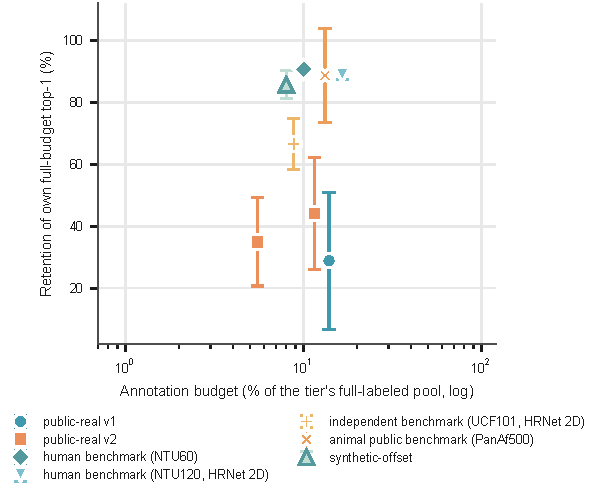
\includegraphics[width=0.76\linewidth]{fig5_budget_retention.pdf}
  \caption{Budget--retention summary: each point plots one tier's PSD pipeline at a labeled-data fraction against its retained full-budget top-1 (error bars: seed std; corrected protocol; the NTU60 error bar, $\pm$ 0.3\,pp, is smaller than its marker). The shaded 85--90\% band is the pre-registered PARTIAL decision band. Tier groups are never connected or pooled; near-coincident budgets are displaced along the log axis (v1 12.8\% shown at 13.9\%, v2 spc4 10.9\% at 11.5\%, synthetic-offset 9.1\% at 8.0\%, UCF101 10\% at 8.8\%, PanAf500 10\% at 13.2\%, NTU120 10\% at 16.5\%); plotted values, error bars, and ordinal axis spacing are unaffected. Retention is high on the human benchmarks under the interim supervised encoder (NTU60 90.7\%; NTU120 88.9\%, plotted; label-free pretext 74.96\%, FAILS, not plotted), on PanAf500 (88.7\% (plotted) at ten seeds; 85.8\% at thirty, interim encoder; 82.5\% label-free, FAILS, not plotted), and on the synthetic-offset tier, but collapses toward chance on the canine public-real tier at 13\%/5.5\% budgets (E7/E7b) and drops to 66.6\% on UCF101 (full-budget reference 23.1\%), bounded by pseudo-label quality, not budget arithmetic.}\label{fig:budget}
\end{figure}

\subsection{Comparison studies}\label{sec:comparison}

\emph{Tag disambiguation:} the reinforcement protocols reuse the tags E1--E3b with an explicit \emph{reinforcement} qualifier: Reinforcement E1 (same-episode zero-retraining bound), Reinforcement E2 (matched-budget three-arm contrast), and Reinforcement E3/E3b (split/addition episode and its labeled-budget ladder). These are distinct from the pipeline-stage experiments E1--E3 of Section~\ref{sec:main-results} (physics-layer representation quality, unsupervised segmentation quality, anchor-guided label expansion).

\paragraph{Implementation-equivalence verification on NTU60.}
Because AimCLR, SMQ, and the self-training machinery are re-implemented in this repository rather than imported, we verify implementation correctness on the human-domain benchmark (NTU RGB+D 60~\citep{shahroudy2016ntu}) before applying the pipeline to animal data. Following the linear-evaluation protocol of AimCLR~\citep{guo2022aimclr} on NTU60 cross-subject, each stream (joint, bone, motion) is pretrained for 300 epochs and evaluated with a frozen encoder and a fully-connected classifier, then fused with the official fixed weights (joint 0.6, bone 0.6, motion 0.4). The re-implementation reaches 74.30\% (joint), 71.51\% (bone), and 67.84\% (motion) top-1, and the three-stream fusion attains \textbf{77.97\% top-1 (95.78\% top-5; $n=16{,}487$)}, exceeding our pre-registered acceptance line of 77.18\% and lying within 0.93\,pp of the 78.9\% reported in the AimCLR paper body. We therefore treat the adapted implementation as equivalent to the official one for the purposes of this study. Throughout, baselines run under shared protocols; the head-to-head comparison below (Table~\ref{tab:h2h}) evaluates re-implemented published methods under an identical budget protocol, while no comparison against published \emph{reported} numbers is claimed (Section~\ref{sec:conclusion}, L13).

\paragraph{E9: low-resource retention on the human benchmark (C6, pre-registered).}
The animal-domain low-resource claim would be weak evidence if it did not generalize, so we pre-registered (PSD-NTU-PREREG-001, frozen before the experiment) a budget-shrinkage test on NTU RGB+D 60 cross-subject~\citep{shahroudy2016ntu}. Holding the frozen epoch-300 joint pretext backbone fixed, a 10\% class-stratified subset of the 40{,}091 training clips in the provider's frame-50 export yields 66.05\% with a linear head alone. Applying the PSD semantic pipeline (anchor-guided clustering with iterated confidence-filtered pseudo-labeling) under the corrected protocol of E7 yields \textbf{67.53\% $\pm$ 0.24} (ten seeds, after a 3-seed initial readout was expanded per the E9-series convention; both readouts released), which is \textbf{90.7\%} of the full-budget linear-probe reference of 74.45\% and clears the pre-registered generalization line of 90\%. The denominator is arm (c)'s linear probe, fixed at protocol freeze; under the three-stream fusion caliber of Section~\ref{sec:comparison} the same arms read 86.6\%. The linear-only arm alone already retains 88.7\% of the reference, so the pipeline's margin is modest: the pseudo-label iteration contributes $+1.48$\,pp over the linear-only arm (every seed arm above it; one-sample $t$ raw $p<10^{-7}$, Holm-corrected $p<10^{-6}$; Wilcoxon raw $p=0.002$, corrected $p=0.012$, under the series-wide eight-test family of Section~\ref{sec:implementation}). The labeled subset is $28\times$ larger than the animal-tier training pool (4{,}009 vs.\ 141 clips). An external semi-supervised baseline (PSD-SSL-BASE-001, frozen before the run) bounds this margin from below in the same harness (same frozen features, same 10\% subset, same evaluation): a Mean-Teacher-style~\citep{tarvainen2017mean} pool-distillation arm (soft pseudo-labels, $\tau{=}0.95$ confidence mask, five teacher--student rounds, ten seeds) reaches \textbf{46.79\% $\pm$ 0.61}, so the PSD pipeline exceeds it by $+20.7$\,pp (10/10 paired seed wins, Wilcoxon raw $p=0.002$, Holm-corrected $p=0.012$), while the baseline's confidence mask admits only 15{,}758 of 36{,}082 pool clips; near-full pool restoration is exactly what the confidence-thresholded baseline cannot do. On the weak-reference domain (UCF101) the same baseline lands at parity with its teacher (14.17\% vs.\ 14.04\%; PSD $+1.2$\,pp, n.s.), so the external-baseline disadvantage tracks the reference-quality gradient. Retention ratios are protocol-dependent (a frozen-probe budget-accuracy curve is flatter by construction than a fine-tuned pipeline's), so this arm supports the pipeline's own budget behavior and is not a comparison against any published method.

Four disclosures bound the reading: the pool adds $\approx$35.4k pseudo-labeled clips per seed (the near-restored training-set size \emph{is} the mechanism), and the gate accepts $\approx$98\% of the pool (the consensus gate is inert on the numeric NTU taxonomy), so this arm cannot separate filter quality from pool-size restoration (Section~\ref{sec:conclusion}, L11); the stopping rule is disabled on this tier, and pool precision against the official labels ($\approx$0.69) is a post-hoc diagnostic only; the 10\% subset is a single stratified draw (seed 42), so the $\pm$ 0.24 spread covers self-training seeds but not subset resampling; a post-hoc diagnostic redrawing the subset under four alternative seeds places the linear arm's spread at 65.62\% $\pm$ 0.48 (original 66.05\%, within one resample std; the decoupled arm's subset sensitivity is not measured); and the final head uses StandardScaler + logistic regression (tol $10^{-3}$) with the self-training head on GPU (scale adaptations, otherwise identical to E7).

\paragraph{Head-to-head against published methods under the identical budget protocol.}
The retention study above measures PSD against internal references; to situate the same arms against published methods, two published-method baselines are run in the identical harness on NTU60 cross-subject (Table~\ref{tab:h2h}): the AimCLR linear-evaluation arm (joint stream, official linear-probe recipe; the re-implementation verified above, with in-house pretext weights trained by the official recipe because the official released checkpoint was unreachable) and a supervised ST-GCN trained end-to-end on labels (reduced capacity: 16 hidden channels, 0.84M parameters; a deliberate small-capacity configuration for the 8\,GB GPU, so its accuracy is a same-harness supervised reference, not a reproduction of the published full-capacity model). Every arm consumes the same class-stratified subsets (per-class $k{=}\max(1,\mathrm{round}(f\,n_c))$; the 10\% arms on the protocol-frozen seed-42 draw of E9, 4{,}009 clips) or the full 40{,}091-clip training set, and is evaluated on the same 16{,}487-clip validation split; the PSD arms reuse the E9 numbers unchanged. Two lines of evidence support the 10\% ordering. On the protocol-frozen seed-42 draw, the PSD semantic pipeline reaches \textbf{67.53\% $\pm$ 0.24} (ten self-training seeds), above the AimCLR linear arm (\textbf{66.74\% $\pm$ 0.05} over five initialization seeds; $+0.79$\,pp, Welch $t{=}10.1$, raw $p{=}1.1\times10^{-6}$, Holm over the two post-hoc tests of this comparison $p{=}2.3\times10^{-6}$) and the end-to-end supervised arm (\textbf{64.84\% $\pm$ 2.18} over five initialization seeds; $+2.69$\,pp, Welch $p{=}0.051$, not significant, because one of the five initializations diverges to 61.30\% and inflates the arm's variance; the distribution-free Mann--Whitney test is significant at raw $p{=}6.7\times10^{-4}$, Holm-corrected $p{=}1.3\times10^{-3}$), with both published-method baselines landing within 1.3\,pp of the PSD linear head (66.05\%). On two independent stratified redraws of the 10\% subset (seeds 43/44, post-hoc; a single draw cannot separate draw quality from method effect), the ordering PSD $>$ AimCLR $>$ ST-GCN likewise holds on every draw, with PSD margins of $+7.8$/$+7.3$\,pp over AimCLR and $+10.0$/$+9.3$\,pp over ST-GCN. The pipeline itself is draw-sensitive (67.53\% on the frozen draw versus 74.11\% $\pm$ 0.22 and 74.20\% $\pm$ 0.08 on the redraws, with similar pool-restoration fractions, 97.9--98.7\% versus 95.2--96.1\%, so the gap reflects admitted pseudo-label quality rather than pool volume; the mechanism is not resolved and the per-draw diagnostics are released). A post-hoc budget extension on the same seed-42 draw (5\%/20\% columns of Table~\ref{tab:h2h}) shows the pipeline's advantage growing as the budget shrinks: at 5\% labels PSD reaches 74.20\% $\pm$ 0.05 versus 64.12\% (AimCLR linear) and 52.88\% (end-to-end ST-GCN), margins of $+10.1$/$+21.3$\,pp on the identical draw; and at 20\% 74.08\% $\pm$ 0.15 versus 69.62\%/72.83\%. The 10\% cell of the frozen draw sits below the pipeline's own 5\% and 20\% cells; we report this non-monotonicity as observed and do not fit a narrative to it. At full budget the ordering inverts: end-to-end supervised ST-GCN, consuming all 40{,}091 labels, dominates (83.46\%), while the frozen-feature arms cluster at 74.30\%/74.45\% (AimCLR linear / PSD linear probe). Job wall-clock on the same GPU: 2{,}268\,s (AimCLR) and 4{,}444\,s (supervised ST-GCN) for the original two-budget runs, plus a 20-cell robustness matrix (five-seed initialization block, two subset redraws, two budget extensions) of ${\sim}4.5$\,h total. Figure~\ref{fig:h2hbudget} plots the three budget points of Table~\ref{tab:h2h}. The same harness extends to the second benchmark: on NTU120 (E9b 12,000-clip/60-class subset, label-free physics layer), the linear head on the label-free features reads 44.18\% (the AimCLR linear-evaluation arm), the PSD semantic pipeline 43.75\% $\pm$ 1.16 (ten seeds; the $-0.43$\,pp margin of E9b), and end-to-end ST-GCN 36.17\% $\pm$ 1.71 (five initialization seeds): at this budget the frozen-feature arms sit ${\approx}8$\,pp above end-to-end training, reproducing the same-budget E2 pattern on a second benchmark, while the PSD-vs-AimCLR margin vanishes exactly as the label-free saturation analysis of E9b predicts.

\begin{table}[pos=htbp]
\centering
\caption{Head-to-head comparison on NTU60 cross-subject under an identical budget protocol: every arm trains on class-stratified labeled subsets of the same 40,091-clip training pool (per-class $k{=}\max(1,\mathrm{round}(f\,n_c))$; the 10\% arms use the protocol-frozen seed-42 draw of E9, 4{,}009 clips) and is evaluated on the same 16,487-clip validation split. Both published-method baselines are run by us: AimCLR linear evaluation (joint stream; re-implementation verified in the equivalence check, in-house pretext weights) and a reduced-capacity (16 hidden channels, 0.84M parameters) end-to-end supervised ST-GCN, a same-harness reference, not a reproduction of the published full-capacity model. The full-budget PSD reference is the frozen-feature linear probe; the semantic pipeline is not run at full budget. Baseline 10\% cells are means $\pm$ sample std over five initialization seeds (seed-0 runs included); the PSD 10\% cell reuses the E9 ten-self-training-seed readout; the 5\% and 20\% columns are a post-hoc extension on the same seed-42 draw (baselines: seed 0; PSD: three self-training seeds). At 10\% the PSD--AimCLR gap is $+0.79$\,pp (Welch $t{=}10.1$, raw $p{=}1.1\times10^{-6}$, Holm $p{=}2.3\times10^{-6}$) and PSD--ST-GCN is $+2.69$\,pp (Welch $p{=}0.051$, not significant; one divergent initialization at 61.3\%; Mann--Whitney raw $p{=}6.7\times10^{-4}$, Holm $p{=}1.3\times10^{-3}$). Subset-robustness redraws of the 10\% budget (seeds 43/44, post-hoc) preserve the ordering, with PSD margins of $+7.3$ to $+7.8$\,pp over AimCLR. The NTU120 block extends the same harness to the second benchmark under the label-free physics layer (E9b caliber; 10\% protocol-frozen draw); there the linear head on the label-free features already saturates the separable signal (44.18\%), and frozen features beat end-to-end training by ${\approx}8$\,pp (36.17\%).}
\label{tab:h2h}
\footnotesize
\hyphenpenalty=10000
\begin{tabularx}{\linewidth}{>{\raggedright\arraybackslash}X>{\raggedright\arraybackslash}p{1.7cm}>{\raggedright\arraybackslash}p{2.0cm}>{\raggedright\arraybackslash}p{1.7cm}>{\raggedright\arraybackslash}p{1.7cm}}
\hline
Method (NTU60 xsub; final block = NTU120) & 5\% labels & 10\% labels & 20\% labels & Full budget \\
\hline
Supervised ST-GCN, end-to-end (16 hid.\ ch., reduced capacity) & 52.88\% & 64.84\% $\pm$ 2.18 & 72.83\% & 83.46\% \\
AimCLR linear evaluation (joint stream, re-impl.) & 64.12\% & 66.74\% $\pm$ 0.05 & 69.62\% & 74.30\% \\
PSD linear head on frozen features (E9) & 63.30\% & 66.05\% & 68.79\% & 74.45\% \\
PSD semantic pipeline (E9 protocol) & 74.20\% $\pm$ 0.05 & 67.53\% $\pm$ 0.24 & 74.08\% $\pm$ 0.15 & -- \\
\hline
\multicolumn{5}{l}{\emph{NTU120 (E9b 12{,}000-clip/60-class subset; label-free physics layer; 10\% protocol-frozen draw; same harness)}} \\
Supervised ST-GCN, end-to-end (16 hid.\ ch., reduced capacity; 5 init.\ seeds) & -- & 36.17\% $\pm$ 1.71 & -- & -- \\
Linear head on the label-free features (= AimCLR linear evaluation; E9b) & -- & 44.18\% & -- & -- \\
PSD semantic pipeline (E9b protocol; 10 seeds) & -- & 43.75\% $\pm$ 1.16 & -- & -- \\
\hline
\end{tabularx}
\end{table}

\begin{figure}[pos=htbp]
  \centering
  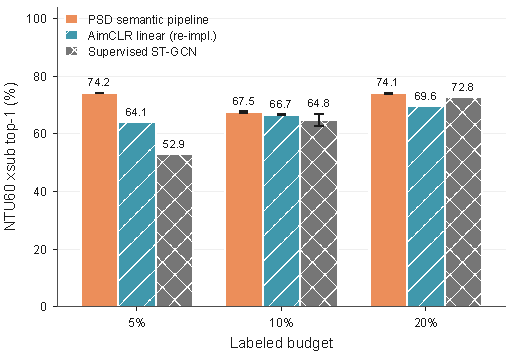
\includegraphics[width=0.76\linewidth]{fig7_h2h_budget.pdf}
  \caption{Head-to-head budget curve on NTU60 xsub (the harness of Table~\ref{tab:h2h}): top-1 of the PSD semantic pipeline, the AimCLR linear arm, and the end-to-end supervised ST-GCN at 5\%, 10\%, and 20\% class-stratified labeled budgets (bar means; error bars only where the released arm carries seed dispersion). The 10\% cells sit on the protocol-frozen seed-42 draw of E9; the 5\% and 20\% cells are the post-hoc extension on the same draw. Read the ordering across budgets from the figure; exact values, dispersions, and significance tests are in Table~\ref{tab:h2h} and the accompanying text.}\label{fig:h2hbudget}
\end{figure}

\paragraph{E9b/E9c: cross-domain retention gradient (pre-registered).}
To test whether the retention behavior is a property of the pipeline rather than of one benchmark, we pre-registered two further replications (PSD-NTU120-PREREG-001 and PSD-UCF101-PREREG-001, frozen before any run). On NTU RGB+D 120~\citep{liu2020ntu}, the official 3D-skeleton application was denied, so the replication uses the PYSKL-release HRNet 2D joint annotations (same video source and official labels, different extractor). It consumes a 12{,}000-clip, 60-class subset of the PYSKL NTU120 export, a caliber held identical across all arms (per-tier calibers in the supplementary material). The pretext is a joint-level MLP over all joint coordinates (80 epochs, frozen 256-d penultimate); this is a disclosed deviation from the frozen ST-GCN plan, adopted so one pretext architecture runs unchanged across both 17-joint benchmarks, with backbone quality absorbed by the full-budget reference arm. A supervision disclosure added in this revision: the interim MLP was trained with cross-entropy on the \emph{full} training labels, so on these tiers the frozen encoder is supervised, unlike the label-free contrastive physics layer used on NTU60 and claimed by the framework. At a 10\% stratified budget (ten seeds, after a 3-seed initial readout was expanded per the E9-series convention, adopted 2026-09-07 as a dated amendment; both readouts released; spreads cover self-training seeds but not subset resampling), the pipeline reaches \textbf{48.3\% $\pm$ 0.8} top-1 against the 10\%-linear arm's 45.4\% ($+2.9$\,pp; every seed arm above the linear arm). Significance tests use one-sample $t$ ($t{=}12.0$, raw $p<10^{-5}$) and Wilcoxon (raw $p=0.002$), Holm-corrected over the series-wide eight-test family (Section~\ref{sec:implementation}): corrected $p<10^{-5}$ and $0.012$, and conclusions are invariant to any narrower family choice. Retention against the full-budget reference's 54.3\% is \textbf{88.9\%, in the pre-registered PARTIAL band (85--90\%)}. A protocol-return amendment (2026-11-17) then executed the pre-registered physics layer itself on the identical 12{,}000-clip caliber: a from-scratch \emph{label-free} AimCLR pretext (ST-GCN base, 150 epochs, single joint stream, exactly as frozen in PSD-NTU120-PREREG-001; the 17-joint HRNet topology mapped into a fixed 16-active-slot arrangement on the 25-node NTU graph, nine dead slots, slot table in the supplementary material). Its full-budget reference (58.37\%) exceeds the interim encoder's (54.34\%), but the semantic pipeline reads 43.75\% $\pm$ 1.16 (ten seeds 42--51, completed in two sessions after a host-resource interruption; both logs released) against a 44.18\% linear head, a $-0.43$\,pp margin, for \textbf{74.96\% retention, FAILS}. Under the label-free pretext the linear head already saturates the separable signal at this budget, and pseudo-labeling adds nothing. Both readouts are released; neither supersedes the other (the interim verdict is the record of the executed-deviation protocol, the protocol-return is the record of the pre-registered one). On UCF101~\citep{soomro2012ucf101}, an independent third domain (YouTube-sourced video, 101 classes, HRNet 2D skeletons~\citep{sun2019hrnet}), the replication consumes a 10{,}000-clip subset under the same caliber (identical across arms; the official split-1 validation fold comprises 463 clips, part of the reported caliber). The same protocol yields \textbf{15.4\% $\pm$ 1.9} against a 14.0\% linear arm ($+1.4$\,pp; 8/10 seed arms above) and a 23.1\% reference; both tests are direction-consistent but neither significant (raw $t$ $p=0.049$, Wilcoxon raw $p=0.053$, Holm-corrected $p=0.141$ for both): \textbf{66.6\% retention, below the 85\% line, reported as a negative boundary}. The label-free protocol-return (2026-11-18) executes the pre-registered pretext on the identical 10{,}000-clip caliber: full-budget reference 19.87\% (vs.\ the interim encoder's 23.11\%), 10\% linear head 9.94\%, semantic pipeline 10.15\% $\pm$ 2.04 (ten seeds 42--51), a $+0.2$\,pp margin, for \textbf{51.09\% retention, FAILS}; both readouts are released. The external SSL baseline (Amendment 1 of PSD-SSL-BASE-001) extends to this domain: the Mean-Teacher arm reaches \textbf{14.17\% $\pm$ 0.87}, parity with its own teacher, the linear head (14.04\%), so the PSD pipeline's advantage over it is $+1.2$\,pp (8/10 wins, Wilcoxon raw $p=0.047$, Holm-corrected $p=0.141$; not significant). Where the full-budget reference is weak, confidence-thresholded pool distillation adds nothing: the same pretext-learnability gradient, now observed on the external-baseline axis.

Read together, the cross-domain points form a monotone gradient within the E9 series (NTU60 under the label-free AimCLR pretext; NTU120 and UCF101 under the interim supervised encoder). Retention falls from 90.7\% on NTU60 to 88.9\% on NTU120 and 66.6\% on UCF101 as the full-budget reference quality falls from 74.45\% to 54.3\% and 23.1\% (all E9-protocol linear-probe references; the AimCLR official-protocol re-implementation of the NTU60 reference is 74.30\%, Section~\ref{sec:comparison}). This indicates that what the frozen pretext learned about class-separable structure, not the budget arithmetic, bounds how far pseudo-label self-training can be stretched. The protocol returns isolate the encoder factor within tier. On NTU120, swapping the interim supervised encoder for the pre-registered label-free pretext raises the full-budget reference (54.34\% $\to$ 58.37\%) yet lowers retention (88.9\% $\to$ 74.96\%): on the label-free features the 10\% linear head already saturates the separable signal (44.18\%), so the pseudo-label pipeline's margin vanishes ($-0.43$\,pp). On UCF101 the same swap lowers both (reference 23.11\% $\to$ 19.87\%; retention 66.6\% $\to$ 51.09\%). On PanAf500 the swap raises the reference (60.0\% $\to$ 64.0\%) yet lowers retention (85.8\% $\to$ 82.5\%), the pipeline falling $7.2$\,pp below its own 10\% linear head. Under the single pre-registered label-free layer the ordering is monotone across all four executed tiers: retention 90.7\% $\to$ 82.5\% $\to$ 74.96\% $\to$ 51.09\% tracks reference quality 74.45\% $\to$ 64.0\% $\to$ 58.37\% $\to$ 19.87\% (NTU60/PanAf500/NTU120/UCF101). Retention is therefore a property of the physics layer's feature geometry, not of reference quality alone. The gradient claim is accordingly conditioned: \emph{within a fixed physics layer}, retention is monotone in full-budget linear-probe reference quality, with the high band (85--90\%) holding where the reference is separable and collapse where it is not. Any tier whose reference is strongly separable ($\geq$70\%) yet retains $<85\%$ at a 10\% budget under a fixed layer would break it; the pre-registered working-dog pilot is designed to supply such a test. This is the same mechanism boundary diagnosed on the canine tier (E7; the alignment analysis of Section~\ref{sec:conclusion}, L9), now observed on three additional public benchmarks. The low-resource claim is therefore scoped to tiers whose pretext features support linear separability at full budget, and the retention line is not claimed as a domain-universal property.

\paragraph{E9d: first animal-domain public benchmark (PanAf500, pre-registered).}
The mechanism boundary above predicts that retention depends on what the pretext learned, not on taxonomy, so it should extend beyond the human domain wherever a public animal benchmark exists. PanAf500 (great-ape natural behavior, in-the-wild video, 500 clips with official splits and nine behavior classes) is the public animal benchmark we could identify, and we pre-registered its budget-shrinkage test (PSD-PANAF-PREREG-001, frozen before any run) \emph{after} the E9b/c gradient was observable but \emph{before} the PanAf run executed. Its full-budget reference (60.0\%) lies below the $\geq$70\% falsifier threshold of the gradient's strong form, so this run is a directional consistency check rather than a potential falsifier: the observed retention (88.7\% at the pre-registered ten seeds; 85.8\% at the thirty-seed amendment below; both in the PARTIAL band) is consistent with the high band predicted for separable references. Skeletons are model-extracted: a YOLO11x-pose model fine-tuned on the ape subset of AP-10K (17-keypoint topology mapped onto the 24-slot PanAf extraction layout with seven dead slots; 17 active of 24 (an extraction-layout count), distinct from the 16-active/nine-dead arrangement of the 25-node NTU export mapping in the E9b/E9c calibration above) infers keypoints on bbox-cropped frames (82.1\% mean frame detection, 0.59 mean confidence; extraction noise enters all arms equally). Pretext, arms, budget, and decision rule mirror E9b/E9c. At a 10\% stratified budget (ten seeds), the pipeline reaches \textbf{53.2\% $\pm$ 9.1} against the 10\%-linear arm's 52.0\% and the full-budget reference's 60.0\%, for \textbf{88.7\% retention, in the pre-registered PARTIAL band} (a 3-seed early readout of 93.3\% fell into the CONFIRMS band and is superseded by the 10-seed number under the frozen rule; both released). The test split (75 clips, held out of the decision rule) yields 56\% as a non-decision secondary number. Two disclosures bound the reading: the nine-class space is long-tailed (three classes have $\le$7 clips; five classes contribute a single seed clip at the 10\% budget), inflating seed variance; and behavior labels are frame-level annotations majority-voted to clip level, the same coarse granularity diagnosed on the canine tier. PanAf500 completes the cross-domain picture at four points spanning two kingdoms. Under the interim supervised encoder, retention stays in the high band wherever the full-budget reference is separable (NTU60 90.7\%, NTU120 88.9\%, PanAf500 85.8\% at thirty seeds) and collapses where it is not (UCF101 66.6\%, reference 23.1\%). Executing the pre-registered label-free pretext on NTU120, despite its \emph{higher} reference (58.37\%), drops retention to 75.0\% (FAILS; rounded from the 74.96\% readout above); on UCF101 it lowers both the reference (23.1\% $\to$ 19.9\%) and the retention (66.6\% $\to$ 51.1\%, the rounded 51.09\%). On PanAf500 (2026-11-18 protocol return on the identical caliber; the PSD24 quadruped layout mapped to the same 16-active-slot arrangement, slot table in the supplementary material), the same swap raises the reference (60.0\% $\to$ 64.0\%) yet drops retention to \textbf{82.5\%, FAILS} (pipeline 52.8\% $\pm$ 9.6, ten seeds 42--51, against a 60.0\% linear head; interim readout 85.8\%, PARTIAL). This isolates the encoder's feature geometry as the binding factor (Section~\ref{sec:comparison}); budget retention is a property of pretext learnability, not of species or domain. The PanAf pipeline-vs-linear gap is not carried by the evidence at any tested power: at ten seeds it reads $+1.2$\,pp with 5/10 seed wins. A post-hoc seed expansion to thirty seeds (Amendment 2 of PSD-PANAF-PREREG-001, frozen before the run; seeds 42--71, both readouts released) gives 51.5\% $\pm$ 8.6 against the same linear arm (13/30 wins, 3 ties, Wilcoxon $p=0.54$), retention 85.8\%, verdict unchanged. The gap is therefore reported as directional only, and even $n{=}30$ does not separate the arms on this long-tailed nine-class space; as on NTU60, PanAf's retention is carried predominantly by the frozen-feature linear head, and no pipeline advantage is claimed on this tier.


\paragraph{E6-real-2: backbone-scale replication with matched solvers (pre-registered).}
TRANS-001's coupled arm retrains in $\approx$35\,s, so its cost endpoint was arithmetically unpassable: the replication could not have confirmed the cost claim at that scale. A second pre-registered replication (PSD-NTU-TRANS-002, frozen before the run; same $\mathcal{Y}\to\mathcal{Y}'$ merge, 60$\to$49 classes) therefore scales the backbone to the full ST-GCN of the equivalence verification and adds a third arm that decouples the two confounds TRANS-001 carried: the matched-solver arm (M) retrains a linear head on the coupled arm's own penultimate features with the decoupled arm's solver, isolating representation quality from retraining cost. As in TRANS-001, this merge-type transition admits the zero-retraining upper bound of Section~\ref{ssec:boundary}; the control is reported in Table~\ref{tab:attribution-controls}, whose same-episode ($60\to49$) bound rows carry the executed E1 reinforcement measurement (inference-only: 68.04\% rename-oracle upper / 67.97\% argmax-vote lower at the 10\% labeled head budget, zero retraining; protocol in the supplementary material). Full budget (40,091 clips, seeds 42--44): the coupled arm retrains in a median of 9897\,s against the decoupled head's 626\,s (15.8$\times$; verdict \textbf{PARTIAL} per the frozen rule), accuracy 79.8\% (coupled) vs 75.3\% (decoupled, gap $-4.5$\,pp). A first run at the nominal scaled learning rate collapsed to a constant predictor mid-training on all three seeds (NaN) and was discarded under a NaN watchdog added to the protocol; the reported run uses half the linear-scaled learning rate. All three coupled-arm seeds include host-restart segments; wall-clock is the sum of contributing segments per seed, with the per-segment decomposition in the released artifact. The verdict is robust to the accounting: a final-segment-only bound (6.2$\times$) still clears the $3\times$ line. At the 10\% budget the same replication reads 32.5$\times$ (coupled 1520\,s vs decoupled 47\,s; ratio on unrounded seconds) with a $+2.6$\,pp decoupled advantage (\textbf{PARTIAL} at the 10\% tier). A dated addendum (PSD-NTU-TRANS-002-MEXP, frozen before the expansion ran) replicated the matched-solver comparison over ten seeds (42--51; the three seeds above reused unchanged): the matched-solver arm exceeds the coupled arm on every seed (mean 82.6\% vs 79.7\% over ten seeds; the three-seed frozen-budget comparison above reads 82.6\% vs 79.8\%; $+2.9$\,pp; paired Wilcoxon $p=0.002$, sign test 10/10; two-test addendum family, Holm-adjusted $p=0.004$). End-to-end training under-exploits its own representation, and the frozen cost-ratio verdict is unaffected. A CIL-flavored reference adapted to this episode (LwF-style distillation from the $\mathcal{Y}$-era head with merge-aggregated targets plus old-class replay; protocol and adaptation freedom in the supplementary material) lands between the bound and the coupled arm: \textbf{68.6\% $\pm$ 0.4} at the 10\% labeled head budget and \textbf{72.9\% $\pm$ 0.04} at the full budget (three seeds), comparable to the decoupled rebuild at 10\% (67.6\%) and below it at the full budget (75.3\%), so a CIL-style alternative does not dominate the decoupled structure where the retraining cost is actually saved.

\paragraph{Reinforcement E3: residual value on a split/addition transition (specified in advance, same-day).}
The merge replications above exercise transitions that a frozen $\mathcal{Y}$-era model can absorb without any new supervision; the complementary question is what decoupling is worth when the transition \emph{requires} new supervision. On the synthetic tier, a split/addition episode ($\mathcal{Y}\to\mathcal{Y}'$: $22\to29$ classes, where three parents each split into two children whose parent samples are unavailable in $\mathcal{Y}'$, plus four brand-new classes with no $\mathcal{Y}$-era source; protocol in the supplementary material) probes the new-supervision ladder with four arms (seeds 42--44): the zero-shot remap of the frozen $\mathcal{Y}$-era head cannot name any new class (0\% on the additions; 43.0\% overall), the decoupled semantic rebuild with $k{=}10$ new labels per new class reaches 45.7\% overall (E3's own 50-clip/class pool; the E3b ladder enlarges the pool to 100 clips/class and reads 45.3\% $\pm$ 0.2 at the same nominal $k{=}10$, Table~\ref{tab:kladder}), a frozen head trained on the full $\mathcal{Y}'$ labeling reaches 68.0\%, and coupled full retraining reaches 97.1\%. The decoupled rebuild spends $5\times$ fewer new labels than the coupled arm (100 vs.\ 500) at $3.02\times$ lower median wall-clock (50.6\,s vs.\ 153.0\,s); under the E6 decision rule the episode returns \textbf{PARTIAL}: the cost line is cleared, but the $-51.4$\,pp accuracy gap exits the $\pm2.3$\,pp band. Whether that gap closes as the decoupled arm's label budget grows is the subject of the ladder below.

\paragraph{Reinforcement E3b: labeled-budget ladder on the split/addition episode ($k\in\{10,25,50,100\}$; specified in advance, same-day).}
The ladder holds the E3 episode fixed and grants the decoupled arm exactly $k$ stratified fresh labels per new class (the 19 retained classes keep their $\mathcal{Y}$-era labels via remap), while the coupled and frozen-head arms consume the full $\mathcal{Y}'$ labeling as $k$-independent references (Table~\ref{tab:kladder}; protocol in the supplementary material). Two caliber disclosures: the annotation pool is enlarged from 50 to 100 clips per class so the $k{=}100$ rung is drawable, making $k{=}10$ a trend reference rather than an exact replication of E3; and the coupled and frozen-head arms are $k$-independent, so their three-seed readout is reused at every rung. Every rung is reported as the mean $\pm$ s.d.\ over seeds 42--44; seeds 43--44 at $k\in\{10,25,50\}$ were added by a same-day supplemental run, and the initial single-seed and merged three-seed readouts are both released. The decoupled arm rises monotonically from 45.3\% to 72.4\% but saturates at the frozen-feature ceiling: at $k{=}100$ it coincides with the frozen-head arm (72.4\% vs.\ 71.7\%; same frozen path, same full new-label budget), while the coupled arm holds at 95.9\%$\pm$0.5. The margin never leaves 23.45--50.57\,pp, far outside the $\pm2.3$\,pp parity band, so no critical $k^{\ast}$ exists within the tested range: the residual-value hypothesis is \emph{not supported at any tested budget}. Decoupling's measured value here is confined to label and wall-clock savings (at $k{=}10$: 100 vs.\ 1{,}000 new labels; 92\,s vs.\ 234\,s, seed 42); closing the accuracy gap appears to require adapting the frozen encoder rather than adding labels. Figure~\ref{fig:kladder} plots this ladder readout against the two $k$-independent references and the $\pm2.3$\,pp parity band.

\begin{table}[pos=htbp]
\centering
\caption{Labeled-budget ladder on the synthetic split/addition episode (reinforcement E3b; $22\to29$ classes; episode fixed at seed 42; every cell is the mean $\pm$ s.d.\ over seeds 42--44; the coupled and frozen-head arms consume the full $\mathcal{Y}'$ labeling and are therefore $k$-independent references, identical across rungs). The annotation pool is 100 clips per class, so the $k{=}10$ rung is a trend reference rather than an exact replication of E3. The coupled-minus-decoupled margin stays far outside the $\pm2.3$\,pp parity band at every rung: no critical $k^{\ast}$ exists within the tested range.}
\label{tab:kladder}
\footnotesize
\hyphenpenalty=10000
\begin{tabularx}{\linewidth}{>{\raggedright\arraybackslash}p{2.2cm}>{\raggedright\arraybackslash}p{2.2cm}>{\raggedright\arraybackslash}p{2.0cm}>{\raggedright\arraybackslash}p{2.0cm}>{\raggedright\arraybackslash}X}
\hline
New labels per class $k$ (total) & Decoupled rebuild top-1 & Coupled top-1 ($k$-indep.) & Frozen head top-1 ($k$-indep.) & Coupled $-$ decoupled margin \\
\hline
10 (100) & 45.3\% $\pm$ 0.2 & 95.9\% $\pm$ 0.5 & 71.7\% $\pm$ 0.5 & 50.57\,pp \\
25 (250) & 59.1\% $\pm$ 2.5 & 95.9\% $\pm$ 0.5 & 71.7\% $\pm$ 0.5 & 36.78\,pp \\
50 (500) & 65.1\% $\pm$ 1.3 & 95.9\% $\pm$ 0.5 & 71.7\% $\pm$ 0.5 & 30.80\,pp \\
100 (1{,}000) & 72.4\% $\pm$ 0.0 & 95.9\% $\pm$ 0.5 & 71.7\% $\pm$ 0.5 & 23.45\,pp \\
\hline
\end{tabularx}
\end{table}

\begin{figure}[pos=htbp]
  \centering
  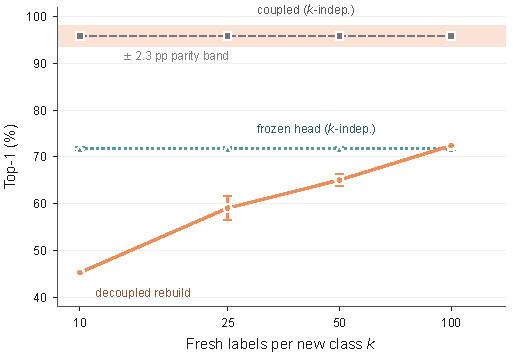
\includegraphics[width=0.76\linewidth]{fig6_kladder.pdf}
  \caption{Labeled-budget ladder on the synthetic split/addition episode (reinforcement E3b; readout of Table~\ref{tab:kladder}): top-1 of the decoupled semantic rebuild as its fresh-label budget $k$ per new class grows (seeds 42--44; error bars: seed s.d.). The coupled and frozen-head arms consume the full $\mathcal{Y}'$ labeling and are drawn as $k$-independent horizontal references; the shaded band is the $\pm2.3$\,pp parity band around the coupled arm. The decoupled arm rises monotonically yet saturates at the frozen-feature ceiling, and its margin to the coupled arm never enters the band; exact per-rung values are in Table~\ref{tab:kladder}.}\label{fig:kladder}
\end{figure}

\paragraph{Segmentation strategy.}
Under the seeds pseudo-ground-truth protocol (Section~\ref{sec:ablation}), motion-word quantization (0.458$\pm$ 0.049) leads the equal-segment-count uniform-window arm (0.399$\pm$ 0.035) and the random-cut null (0.323$\pm$ 0.022), passing all three pre-registered gates; a fixed-grid probe (0.453$\pm$ 0.027) is statistically on par, and uniform windows lead on boundary F1 (0.396 vs.\ 0.343). Per the downgraded positioning of SMQ (an auxiliary proposal source), no end-to-end recognition advantage is claimed from these numbers alone; the dedicated downstream ablation (equal-count fixed windows under the identical frozen-feature head) attributes $\Delta = 0.0$ clip-level accuracy to SMQ (Section~\ref{sec:ablation}), and the full end-to-end pipeline attribution remains future work.

\paragraph{End-to-end comparison against training from scratch.}
A five-arm study on the same 12-class protocol (three seeds; full protocol and per-arm numbers in the supplementary material) completes the matrix: under the frozen-head protocol (the usage mode our decoupled design prescribes), the pretrained backbone outperforms a random one by $+8.3$\,pp (35.71\% vs.\ 27.38\%), whereas under \emph{full} fine-tuning the advantage disappears (36.90\% vs.\ 36.90\%; the scratch arm attains the best macro-F1), corroborating the gradient-ablation crossover of Section~\ref{sec:ablation}: past the crossover budget the pretrained prior adds no value \emph{as a fine-tuning initialization}. Every deep arm and a flatten-plus-logistic baseline cluster in a narrow 27--37\% band (random 6.0\%, majority 25.0\%): the tier's ceiling is set by the self-extraction data bottleneck, not by the choice of model. Reference calibers on this tier (33.93/35.71/36.90/37.50/35.42\%) span up to 3.6\,pp, a caliber effect, not a model effect; within-protocol arm comparisons are unaffected.

\paragraph{Scope statements.}
The NTU60 equivalence verification covers the AimCLR pretraining and three-stream fusion protocol; SMQ is validated through pre-registered ablation comparisons rather than against an official baseline protocol (none is published), and the TCL-style self-training is delivered as an equivalent iteration loop since no official implementation exists (Section~\ref{ssec:selftrain}). Two further registered comparisons remain outside the present evaluation and are not claimed anywhere in this paper: the AimCLR++ backbone variant (80.9\% NTU cross-subject per the official repository's linear-evaluation table) as an alternative physics-layer encoder, and exhaustive sweeps over the confidence threshold $\tau$ and cluster count $K$.

\begin{table}[pos=htbp]
\centering
\caption{Main results under the three-tier protocol (plus the public human-domain benchmark used for implementation-equivalence verification). Tiers are never mixed; the real-K9 row is blank because that tier is not exercised (Section~\ref{sec:datasets}); per-class breakdowns accompany the four-class public-real aggregate (Section~\ref{sec:conclusion}); attribution controls are consolidated separately in Table~\ref{tab:attribution-controls}. The synthetic full-budget reference (96.6\%) is a single seed-42 run without dispersion; retention figures using it as denominator inherit that caliber.}
\label{tab:main}
\footnotesize
\hyphenpenalty=10000
\begin{tabularx}{\linewidth}{>{\raggedright\arraybackslash}p{2.7cm}>{\raggedright\arraybackslash}X>{\raggedright\arraybackslash}p{1.2cm}>{\raggedright\arraybackslash}p{4.1cm}}
\hline
Tier & Task / protocol & Metric & Result \\
\hline
Synthetic & 22-class, full budget (matched 50-ep) & top-1 & 96.6\% (single run, seed 42) \\
Synthetic-offset & 22-class, 20-clip warm-start & top-1 & 82.0\% ($\pm$ 4.3) \\
Synthetic & taxonomy transition, decoupled vs.\ full & wall-clock & 31.1\,s vs.\ 188.7\,s ($6.07\times$; $\geq 3\times$ claimed) \\
\hline
Public-real & $k$-NN subject probe (representation) & top-1 & 20.89\% ($2.51\times$ random) \\
Public-real & segmentation IoU (seeds pseudo-GT) & IoU & 0.458 $\pm$ 0.049 \\
Public-real & prototype purity (InterPet4D 7-label seed space) & purity & 0.5339 ($1.61\times$ random; $+4.8$\,pp majority) \\
Public-real & pseudo-label pool precision (round-1 endpoint) & prec. & 0.691 $\pm$ 0.013 (paired first-to-last n.s.) \\
Public-real & 4-class partial, frozen backbone + head & top-1 & 41.5\,$\pm$\,5.9 (3 seeds; best 44.90\%; per-class in Section~\ref{sec:conclusion}, L7) \\
Public-real & 12-class two-arm (warm vs.\ random backbone) & top-1 & 35.71\% vs.\ 27.38\% \\
Public-real & 12-class two-arm under full fine-tuning (null; five-arm study) & top-1 & 36.90\% vs.\ 36.90\% \\
Public-real & end-to-end PSD pipeline @ 13\% budget, corrected pseudo-label protocol (10 seeds) & top-1 & 9.8\% (chance 11.1\%; negative boundary, E7) \\
Public-real & generic-SSL control @ 13\% budget (10 seeds) & top-1 & 15.2\% $\pm$ 5.1 (above pipeline; E7) \\
Public-real (v2 replication) & same corrected protocol, expanded tier @ 2 clips/class (10 seeds) & top-1 & 13.1\% (chance 12.5\%; E7b) \\
\hline
Public human benchmark & NTU60 xsub 3-stream fusion (equivalence) & top-1 & 77.97\% (line: 77.18\%) \\
Public human benchmark & PSD pipeline @ 10\% labels, corrected protocol (E9, retention) & top-1 & 67.5\% (90.7\% of linear-probe ref 74.45\%; line: 90\%, ten seeds) \\
Public human benchmark (HRNet 2D) & NTU120 replication @ 10\% labels, corrected protocol (E9b, retention) & top-1 & 48.3\% interim supervised encoder (88.9\% of probe ref 54.3\%; PARTIAL band 85--90\%, ten seeds); 43.75\% pre-registered label-free pretext (74.96\%, FAILS; Section~\ref{sec:comparison}) \\
Animal public benchmark (PanAf500) & PSD pipeline @ 10\% labels, corrected protocol (E9d, retention) & top-1 & 51.5\% interim supervised encoder (85.8\% of probe ref 60.0\%, thirty seeds; ten-seed readout 53.2\%/88.7\%; PARTIAL band); 52.8\% pre-registered label-free pretext (82.5\%, FAILS; Section~\ref{sec:comparison}) \\
Independent benchmark (HRNet 2D, YouTube) & UCF101 @ 10\% labels, corrected protocol (E9c, retention) & top-1 & 15.4\% (66.6\% of probe ref 23.1\%; negative boundary, ten seeds) \\
\hline
Real-K9 & -- & -- & not exercised in this study \\
\hline
\end{tabularx}
\end{table}

